% !TEX root = ../main.tex

\ldots Also see video attachment

\todo[inline, caption = {Synthesis time as a function to number of actions ?}]{Provide data on how computationally costly/cheap behavior synthesis is. Time vs number of actions?}

\subsection{Synthesis from scratch}

``synthesis\_pickup\_8" demo \ldots

\begin{figure}[t]
	\centering
	\begin{subfigure}[b]{0.99\columnwidth}
	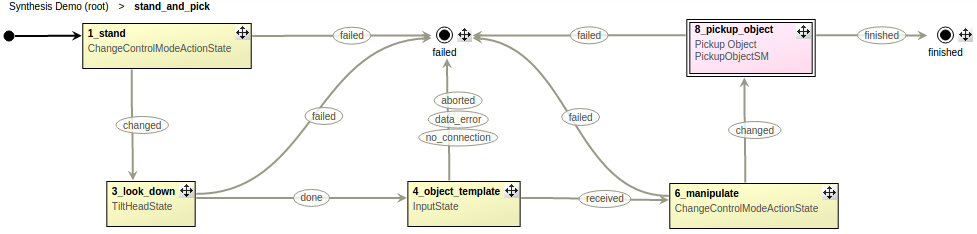
\includegraphics[width=0.99\columnwidth,clip]{./img/stand_and_pick_sm.png}
	\caption{The state machine synthesized for the task $\mathcal{I} = \{ \mathtt{stand\_prep} \}$ and $\mathcal{G} = \{ \mathtt{look\_down}, \mathtt{pickup\_object} \}$.
	}
	\label{Fig:stand_and_pick_sm}
	\end{subfigure}
	
	\vspace{4 pt}
	\begin{subfigure}[b]{0.95\columnwidth}
	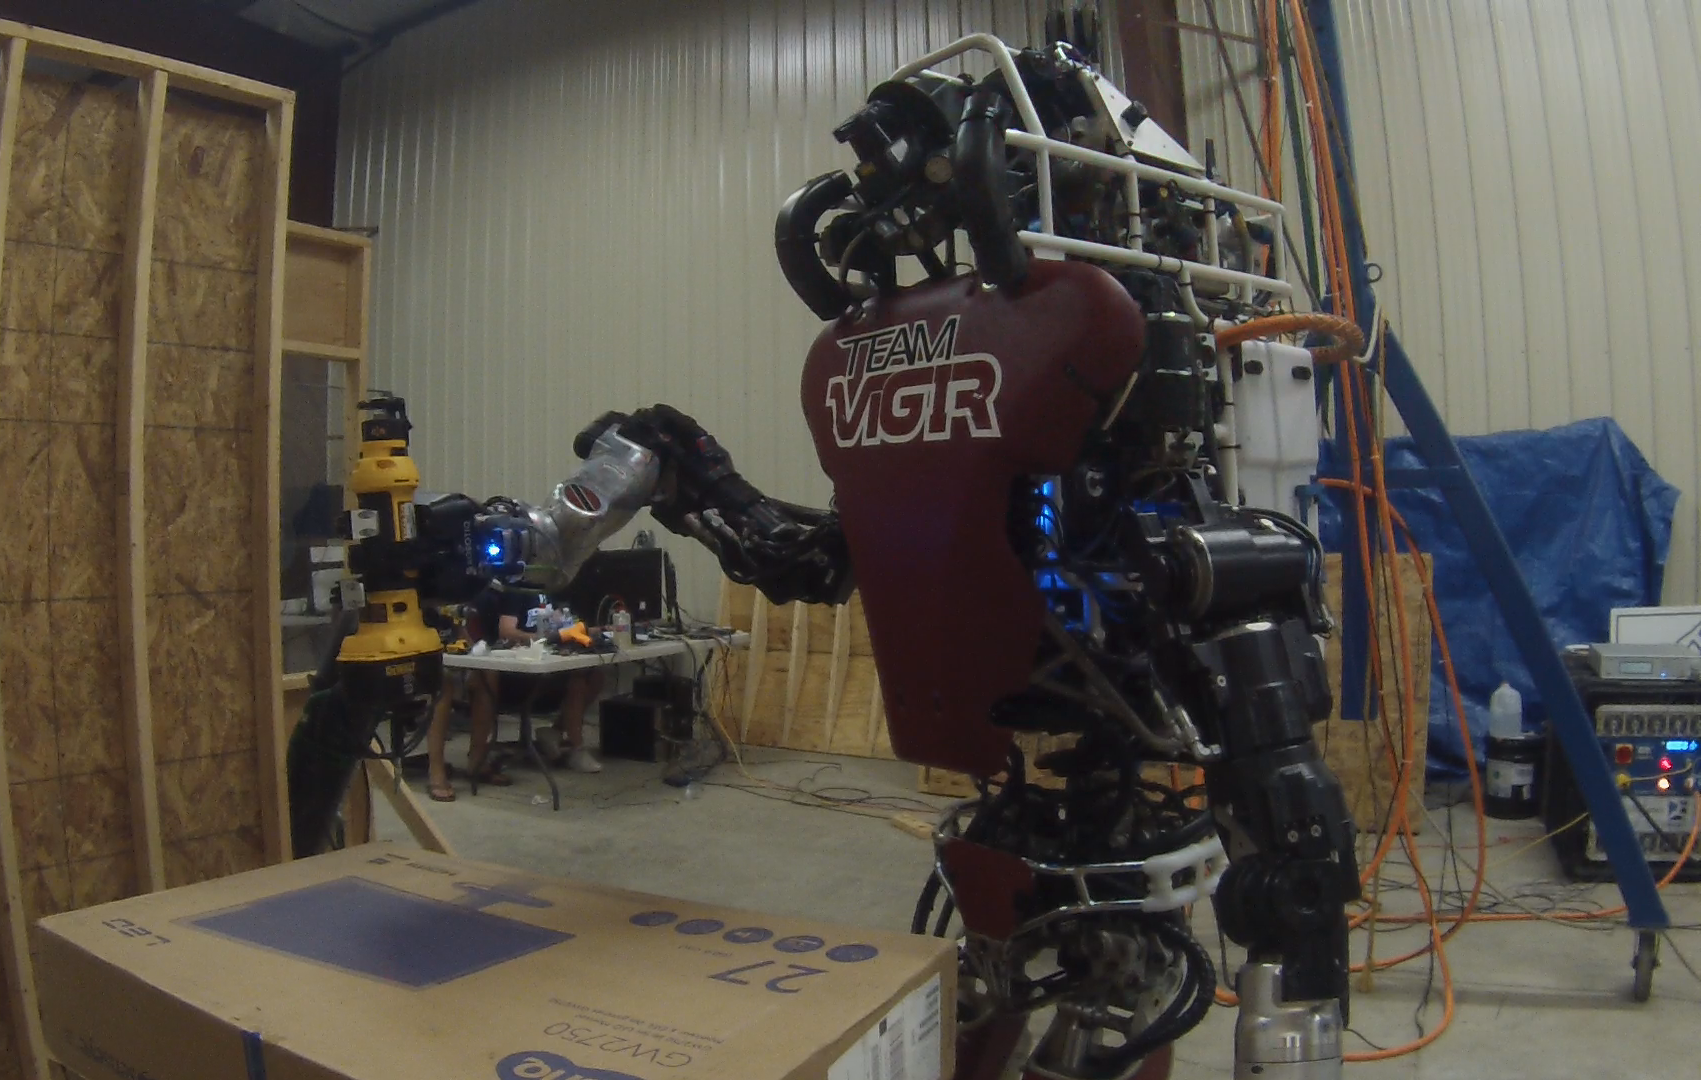
\includegraphics[width=0.99\columnwidth, clip]{./img/stand_and_pick_gopro.png}
	\caption{\ldots
	} 
	\label{Fig:runtime2}
	\end{subfigure}
	\caption{These correspond to the first part of the video attachment.
	}
	\label{Fig:stand_and_pick_demo}
\end{figure}

\todo[inline, caption = {Show generated LTL formulas for synthesis demo}]{Upload the full LTL specification for the ``stand and pick" demo online and add link?}

\subsection{Synthesis on-the-fly}

``synthesis\_runtime\_4" demo \ldots

\begin{figure}[t]
	\centering
	\begin{subfigure}[b]{0.99\columnwidth}
	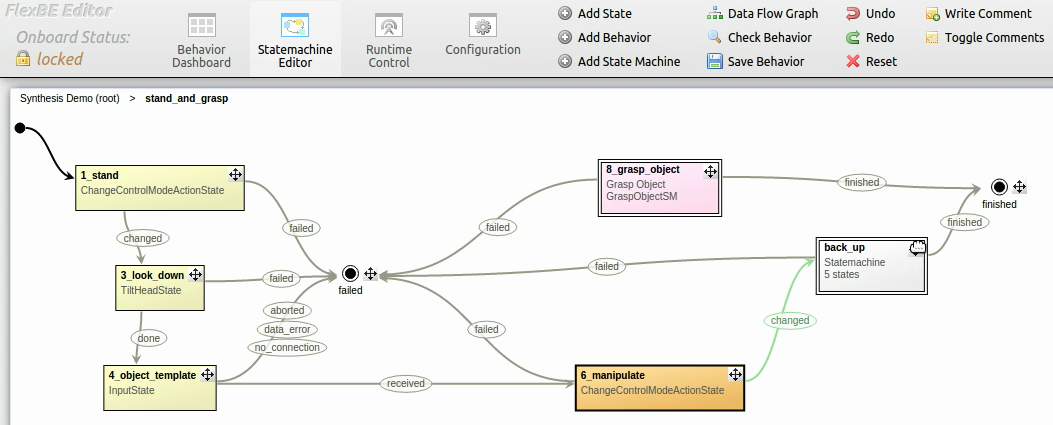
\includegraphics[width=0.99\columnwidth, clip]{./img/synthesis_runtime_connect_sm.png}
	\caption{\ldots
	} 
	\label{Fig:runtime1}
	\end{subfigure}
	
	\vspace{4 pt}
	\begin{subfigure}[b]{0.99\columnwidth}
	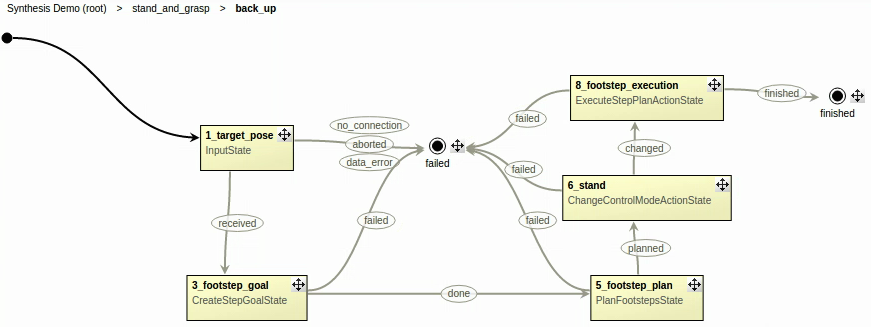
\includegraphics[width=0.99\columnwidth, clip]{./img/synthesis_runtime_synthesized_sm.png}
	\caption{The state machine was synthesized from $\mathcal{I} = \{ \mathtt{manipulate} \}$ and $\mathcal{G} = \{ \mathtt{footstep\_execution} \}$.
	} 
	\label{Fig:runtime2}
	\end{subfigure}
	\caption{Snapshots from \ldots They correspond to the second part of the video attachment.
	}
	\label{Fig:synthesis_runtime_demo}
\end{figure}

% END